\documentclass{article}
\usepackage[a4paper]{geometry}
\usepackage{fancyhdr}
\usepackage{multicol} 
\usepackage{amsmath} 
\usepackage{amssymb} 
\usepackage{tikz}
\pagestyle{fancy}
\lhead{Integrale}
\rhead{April 2025 - August 2025}
\begin{document} 
 
\newcommand{\bitem}[1]{\text{\textbf{#1}}} 
\newcommand{\interndx}[1]{\,\mathrm{d}{#1}} 
\newcommand{\dx}{\interndx{x}}
\newcommand{\dt}{\interndx{t}} 
 
\section{Stammfunktionen}
\begin{minipage}{\dimexpr\linewidth-5cm} 
Eine \emph{Stammfunktion} $F(x)$ von $f(x)$ stellt das Gegenteil der Ableitung dar, sodass $F'(x)=f(x)$. Dementsprechend kann auch überprüft werden, ob ein gegebenes oder gefundenes $F(x)$ tatsächlich die Stammfunktion einer $f(x)$ ist, indem ersteres abgeleitet wird. Die Notation zum bestimmen der Stammfunktion von $f(x)$ ist dabei ein \emph{unbestimmtes Integral}
\[
 \int f(x) \,\mathrm{d}x = F(x) + C
\] 
\end{minipage}
\hfill
\begin{minipage}{5cm}
 \center
 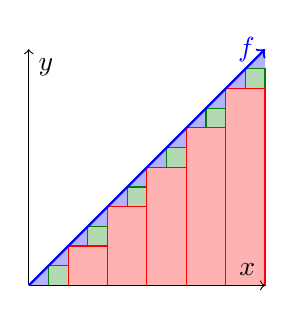
\begin{tikzpicture}
  \fill[blue!30] (0,0) -- (3,3) -- (3, 0) -- cycle;
  \draw[green!50!black, fill=green!50!black!30] (0.25,0.25) rectangle (0.5, 0);
  \draw[green!50!black, fill=green!50!black!30] (0.75,0.75) rectangle (1, 0.5);
  \draw[green!50!black, fill=green!50!black!30] (1.25,1.25) rectangle (1.5, 1);
  \draw[green!50!black, fill=green!50!black!30] (1.75,1.75) rectangle (2, 1.5);
  \draw[green!50!black, fill=green!50!black!30] (2.25,2.25) rectangle (2.5, 2);
  \draw[green!50!black, fill=green!50!black!30] (2.75,2.75) rectangle (3, 2.5);
  
  \draw[red, fill=red!30] (0.5,0.5) rectangle (1, 0);
  \draw[red, fill=red!30] (1,1) rectangle (1.5, 0);
  \draw[red, fill=red!30] (1.5,1.5) rectangle (2, 0);  
  \draw[red, fill=red!30] (2,2) rectangle (2.5, 0);   
  \draw[red, fill=red!30] (2.5,2.5) rectangle (3, 0);
  \draw[->] (0, 0) -- (3, 0) node [above left] {$x$};
  \draw[->] (0, 0) -- (0, 3) node [below right] {$y$};
  \draw[blue, thick, ->] (0, 0) -- (3, 3) node [left] {$f$};
 \end{tikzpicture}   
\end{minipage}
 
\vspace{\baselineskip} \noindent 
Dabei ist $C$ eine konstante, unbekannte Variable, welche hinzugefügt werden muss, weil die gegebene $f$, wie eine Ableitung es nunmal tut, nur die Steigung, nicht den tatsächlichen Wert, von $F$ darstellt. Das $C$ repräsentiert sozusagen jegliche, beim Ableiten verloren gegangene, Konstanten.
 
Das finden der Stammfunktion kann sich durch das annähern des Flächeninhaltes mithilfe von Rechtecke unterhalb der Funktionskurve vorgestellt werden. Geht die Breite der Rechtecke zu $0$, so wird die Annäherung immer genauer.
 
\subsection{Integrationsregeln} 
$\mathrm{n}$ als Konstante 
\begin{multicols}{2} % despite being 1 col this pushed it to the left nicely
 \noindent \begin{align*}
  &\bitem{Summenregel} &&\int f(x) + g(x) \dx &&= \int f(x) \dx + \int g(x) \dx \\ 
  &\bitem{Faktorregel} &&\int n \cdot f(x) \dx &&= n \cdot \int f(x) \dx \\
  &\bitem{Potenzregel} &&\int x^n \dx &&= \frac{1}{n+1}x^{n+1} + C \quad \text{mit} \quad n \in \mathbb{Z} \setminus \{-1; 0\} \\
  &\bitem{Kettenregel} &&\int g(mx+b) \dx &&= \frac{1}{m} G(mx+b) + C \\     
  &\bitem{e-Funktion} &&\int \mathrm{e}^x \dx &&= \mathrm{e}^x + C \\
  &\bitem{$\sin$-Funktion} &&\int \sin x \dx &&= -\cos x + C \\
  &\bitem{$\cos$-Funktion} &&\int \cos x \dx &&= \sin x + C \\
  &\bitem{$\frac{1}{x}$-Funktion} &&\int \frac{1}{x} \dx &&= \ln \lvert x \rvert + C \\
 \end{align*} 
\end{multicols}
 
\section{Integrale}  
Ein \emph{Integral} stellt die Fläche unterhalb einer Kurve dar, wobei Flächen bei $y<0$ auch negativ Zählen. \emph{Bestimmte Integrale} haben, im Gegensatz zur unbestimmten Integralen, dabei eine untere und eine obere Grenze. Das bestimmte Integral der Funktion $f(x)$ mit der unteren Grenze $a$ und der oberen Grenze $b$ folgt der Form 
\[
 \int_a^b f(x) \,\mathrm{d}x
\]
Beim berechnen des Wertes eines Integrals gilt mit $F(x)$ als Stammfunktion der Funktion $f(x)$
\[
 \int_a^b f(x) \dx =
 F(x) \,\Bigr|_a^b =
 F(b) - F(a)
\] 
Weil hier im endeffekt $C-C=0$ gerechnet wird, ist bei bestimmente Integralen das $C$ irrelevant.
 
\subsection{Bestände} 
Gibt die Funktion $f(x)$ eine Veränderung eines Bestandes an und hat eine Einheit dessen Nenner auch die einheit von $x$ darstellt, wie dass Beispielsweise $f(x)$ die Flussmenge von Wasser in $\mathrm{Liter} \over \text{Minute}$ zur $\text{Minute } x$ angibt, so ist ist die Einheit der Stammfunktion der Zähler von der Einheit von $f(x)$. Im Beispiel wäre $F(x)$ dann in $\text{Liter}$ gemessen. Somit ist die Veränderung des Bestandes zwischen Zeitpunkt $a$ und $b$ dann
\[
 \int_a^b f(x) \dx
\]
Ist bekannt, dass der Bestand bei $t_0$ $b_0$ ist, so ist offensichtlich der bestand zum Zeitpunkt $x$
\[
 b_0 + \int_{t_0}^x f(t) \dt
\]
 
\subsection{Integralfunktionen} 
Eine Integralfunktion $I_a(x)$ von $f(x)$ ist eine Funktion der Form
\[
 I_a(x) = \int_a^x f(t) \dt = F(x) - F(a)
\]
Somit gibt sie bei $x$ die Fläche unter der Kurve von $f(x)$ oder die Veränderung von $F(x)$ seit $a$ an und ihr Ergebniss kann genau wie Integral mit den Grenzen $a$ und $x$ als eine Bestands(veränderung) oder als ein Flächeninhalt interpretiert werden.
 
\subsection{Flächeninhalte}
Weil der Flächeninhalt, im Gegensatz zur Fläche, immer positiv ist, auch wenn $y<0$, muss der Betrag genommen oder die Grenzen getauscht werden, sodass der Wert des Integrals genauso immer positiv ist. 
 
\subsection{Flächeninhalte zwischen mehreren Funktionen}
% TODO: tikz 
Die Fläche zwischen mehrere Funktionen stellt das Integral der Differenz beider Funktionen dar. Dabei muss darauf geachtet werden, dass zu jedem Zeitpunkt die Funktion mit dem kleineren Wert von der Funktion mit dem größeren Wert subtrahiert wird. Wechselt sich dies, muss es in ein neues Integral geteilt werden. Die Schnittpunkte beider Funktionen werden dabei generell als Grenzen verwendet, solange keine anderen vorgegeben sind. 
 
\subsection{Uneigentliche Integrale}
Uneigentliche Integrale sind bestimmte Integrale, welche an mindestens einer ihrer Grenzen nicht definiert sind. Dies kann daran liegen, dass die obere oder untere Grenze bei $\infty$ oder $-\infty$ liegt, dann ist es ein uneigentliches Integral erster Art. Bei der zweiten Art eines uneigentlichen Integrals sind alle Grenzen gegeben, nur die Funktion ist bei mindestens einer der Grenzen nicht definiert. \newline
Gelöst werden uneigentliche Integrale, indem die undefinierte Stelle durch eine Variable $u$ ersetzt wird, welche in einem zum Limit der eigentlichen Grenze geht. Beispielsweise
\[
 \int_a^\infty f(x)\,\mathrm{d}x =
 \lim_{u \to \infty} \int_a^u f(x)\,\mathrm{d}x
\]
Wenn das Limit unendlich ist oder nicht existiert, existiert das gesamte Integral nicht. \newline 
Sind beide Grenzen undefiniert, wird das Integral in zwei uneigentliche Integrale, welche jeweils nur eine undefinierte Grenze haben, aufgeteilt. Dabei muss die Hilfsvariable $c$ zwischen $a$ und $b$ sein.
\[
 \int_{-\infty}^\infty f(x)\,\mathrm{d}x =
 \lim_{u \to -\infty} \int_u^c f(x)\,\mathrm{d}x + 
 \lim_{u \to \infty} \int_c^u f(x)\,\mathrm{d}x
\]
Diese beiden uneigentlichen Integrale können nun problemlos berechnet werden.  
 
\subsection{Rotationskörper}
Weil ein Volumen $V$ das Integral der Flächen $A$ ist und die Fläche einer Rotation eines Stabs mit der Länge $f(x)$ einen Kreis mit der Radius $r=f(x)$ darstellt, für welchen $A=\pi r^2$, gilt, ist
\[V = \pi \cdot \int_a^b (f(x))^2 \dx\]
Die Einheit ist, solange keine andere im Kontext der Aufgabe angegeben ist, VE (Volumeneinheiten). 
  
\subsection{Bogenlängen}
% TODO: tikz um das konzept zu erkären 
Die Bogenlänge einer Funktion, die Länge der Kurve der Funktion innerhalb eines gegebenen Bereiches, kann als Summe der Längen mehrer Hypothenusen von Dreiecken, dessen Kathethen $\Delta x$ und $\Delta y = f'(x) \Delta x$ sind bestimmt werden, wobei aus dem Satz von Pythagoras folgt, dass für Kathetenlängen $l = \sqrt{\Delta x^2 + \Delta y^2}$ gilt.
Geht $\Delta x \to 0$, ist die Bogenlänge die Summe unendlich vieler unendlick kleiner Hypothenusen, sodass sie als Integral berechnet wird
\[l = \int_a^b \sqrt{1+(f'(x))^2} \dx\]   
 
\end{document}
 
 
 
 
